\documentclass[aspectratio=169]{beamer}

\mode<presentation>
{
  \usetheme{Singapore}
  \usecolortheme{default}
  \usefonttheme{default}
  \setbeamertemplate{navigation symbols}{}
  \setbeamertemplate{caption}[numbered]
  \setbeamertemplate{footline}[frame number]
}

\usepackage[french]{babel}
\usepackage[T1]{fontenc}
\usepackage[utf8]{inputenc}
\usepackage{tikz-qtree}
\usepackage[thinlines]{easytable}
\usepackage{siunitx}
\usepackage{calc}
\usepackage{multicol}
\usepackage{graphicx}
\usepackage{xcolor}
\usepackage{textcomp}
\usepackage[backend=biber]{biblatex}
\addbibresource{synthese.bib}
\usetikzlibrary{arrows}

\title{Synthèse de mi parcours}
\author{Thibault de Boutray, Louis Vignier}
\institute{CentraleSupélec}

\AtBeginSection[]
{
  \begin{frame}
  \frametitle{Sommaire}
  \tableofcontents[currentsection]
  \end{frame}
}

\begin{document}

\begin{frame}
  \titlepage
\end{frame}

\begin{frame}{Plan}
  \tableofcontents
\end{frame}

\section{Présentation du sujet}

\subsection{Problème}

\begin{frame}{Problématique}
	Comment vérifier la présence effective d'un utilisateur à un événement, et dans la durée ?
	
	\bigskip
	
	\begin{itemize}
        \item Présence en réunion, en cours, à une conférence
        \item Vérification effectuée par le Maître de Conférence (MDC)
	\end{itemize}

\end{frame}

\subsection{Cahier des charges}

\begin{frame}{Assurer la présence d’un utilisateur à un événement}	
    \begin{itemize}
        \item Vérification ponctuelle\pause
        \item Vérification sur la durée complète de l'événement
    \end{itemize}
\end{frame}

\begin{frame}{Propriétés d'utilisation}
    \begin{itemize}
        \item Simple d’utilisation pour les maîtres de conférence\pause
        \item Supporte $\sim$~150 participants\pause
        \item Portée jusqu'à \SI{150}{\meter}\pause
        \item Peu d’actions de la part des participants\pause
        \item Doit pouvoir fonctionner sur une journée entière\pause
        \item Assure la présence effective et unique de l’utilisateur
    \end{itemize}
\end{frame}

\begin{frame}{Propriétés de Privacy}
    \begin{itemize}
        \item Eviter le "flicage" (par ex. suivi non sollicité en arrière-plan)\pause
        \item Respecter la réglementation en vigueur (RGPD)\pause
        \item Avoir un mode "anonyme" avec un simple compte des participants pour réaliser des statistiques (choisi par le MDC)
    \end{itemize}
\end{frame}

\section{Les attaques}

\begin{frame}
    \centering
\begin{tikzpicture}
    % Amphi
    \draw [black, thick, dotted] (0,0) circle [radius=3];
    \node [above] at (0,3) {Amphi};

    % Prof
    \draw [fill] (0,-0.2) circle [radius=0.05];
    \node [above] at (0,-0.2) {Prof};

    \pause

    % Eleve seul
    \draw [fill, gray] (4,0) circle [radius=0.05];
    \node [right, gray] at (4,0) {Élève seul};
    \draw [->, thick, line width=1.2, gray] (3.75,0) -- (0.5,0);
    \node [right, gray] at (6, 2) {Attaque du lit};

    \pause

    % Complicité interne
    \draw [fill, cyan] (1.3, -1.3) circle [radius=0.05];
    \node [above right, cyan] at (1.3, -1.3) {BP};
    \draw [fill, cyan] (3,-3) circle [radius=0.05];
    \node [right, cyan] at (3,-3) {Complicité interne};
    \draw [->, thick, dashed, line width=1.2, cyan] (2.85,-2.85) -- (1.45,-1.45);
    \draw [->, thick, line width=1.2, cyan] (1.15,-1.15) -- (0.35,-0.35);
    \node [right, cyan] at (6, 1) {Attaque relai (complice)};

    \pause

    % Sans complicité
    \draw [fill, orange] (1.3, 1.3) circle [radius=0.05];
    \node [below right, orange] at (1.3, 1.3) {A};
    \draw [fill, orange] (3,3) circle [radius=0.05];
    \node [right, orange] at (3,3) {Sans complicité};
    \draw [->, thick, dashed, line width=1.2, orange] (2.85,2.85) -- (1.45,1.45);
    \draw [->, thick, line width=1.2, orange] (1.15,1.15) -- (0.35,0.35);
    \node [right, orange] at (6, 0) {Attaque relai (tiers abusé)};

    \pause

    % Pokemon
    \draw [red, thick] (-1.3,-1.3) circle [radius=0.5];
    \node [right, red] at (-0.8, -1.3) {BP};
    \draw [fill, red] (-1.1,-1.3) circle [radius=0.05];
    \draw [fill, red] (-1.3,-1.3) circle [radius=0.05];
    \draw [fill, red] (-1.5,-1.3) circle [radius=0.05];
    \draw [fill, red] (-1.3,-1.5) circle [radius=0.05];
    \draw [fill, red] (-1.3,-1.1) circle [radius=0.05];
    \draw [->, thick, line width=1.2, red] (-0.94,-0.94) -- (-0.35,-0.35);
    \node [right, red] at (6, -1) {Attaque Pokemon\texttrademark};

    \pause

    % sybil
    \draw [fill, olive] (-1.3,1.3) circle [radius=0.05];
    \node [above left, olive] at (-1.3, 1.3) {BP};
    \draw [->, thick, line width=1.2, olive] (-1.15,1.35) to [out=15,in=105] (-0.15,0.45);
    \draw [->, thick, line width=1.2, olive] (-1.35,1.15) to [out=255,in=165] (-0.45,0.15);
    \node [right, olive] at (6, -2) {Attaque Sybil};

\end{tikzpicture}

\end{frame}

\section{Protocoles délimiteurs de distance}

\subsection{Présentation}

\begin{frame}{Les Protocoles Délimiteurs de Distance}
Les Distance Bounding Protocols, ou Protocoles Délimiteurs de Distance, sont des protocoles de sécurité qui permettent à un vérificateur $V$ de s'assurer qu'un prouveur $P$ se trouve à une distance bornée et définie de lui-même. \cite{wiki:pdd}

\bigskip

\pause
\begin{itemize}
\item Introduits par Brands \& Chaum, en 1993 \cite{DB1}
\item Détermine la borne supérieure de la distance avec un appareil
\item Calculs basés sur la vitesse de déplacement d'une OEM (30 cm en 1 ns)
\pause
\item Problème : la vitesse de déplacement d'une OEM est proche de celle d'un calcul dans un CPU 
\end{itemize}

\end{frame}

\begin{frame}{Mesure de distance OEM}
    Programme en C++ permettant de tester avec un ping :
    \begin{itemize}
        \item Vers une autre machine
        \item En local
    \end{itemize}

    \bigskip
    
    On s'aperçoit que même en pingant localhost, sur un test de \si{1000} itérations du programme précédent, on obtient une distance minimale estimée à 3 km. 
\end{frame}


\subsection{Attaques}

\begin{frame}{Attaques sur les protocoles délimiteurs de distance}

En 2009, un article formalise les différentes attaques. \cite{attack}

\begin{center}
\begin{tikzpicture}
    % Zone
    \draw [black, thick, dotted] (0,0) circle [radius=2.25];

    % Lecteur
    \draw [fill] (0,0) circle [radius=0.05];
    \node [above] at (0,0.2) {Lecteur};

    \pause

    % Distance fraud
    \draw [fill, gray] (3,0) circle [radius=0.05];
    \node [right, gray] at (3,0) {Tag};
    \draw [->, thick, line width=1.2, gray] (2.75,0) -- (0.5,0);
    \node [right, gray] at (4.5,2) {Distance fraud};

    \pause

    % Mafia fraud
    \draw [fill, cyan] (1.32, -0.44) circle [radius=0.05];
    \node [below, cyan] at (1.32, -0.54) {A};
    \draw [fill, cyan] (3,-1) circle [radius=0.05];
    \node [right, cyan] at (3,-1) {Tag};
    \draw [->, thick, dashed, line width=1.2, cyan] (2.79,-0.93) -- (1.51,-0.5);
    \draw [->, thick, line width=1.2, cyan] (1.1,-0.37) -- (0.47,-0.16);
    \node [right, cyan] at (4.5,1) {Mafia fraud};

    \pause

    % Terrorist fraud
    \draw [fill, orange] (1.32, 0.44) circle [radius=0.05];
    \node [above, orange] at (1.32, 0.54) {A};

    \draw [fill, orange] (3,1) circle [radius=0.05];
    \node [right, orange] at (3,1) {Tag};
    \draw [->, thick, dashed, line width=1.2, orange] (2.79,0.93) -- (1.51,0.5);
    \draw [->, thick, line width=1.2, orange] (1.1,0.37) -- (0.47,0.16);
    \node [right, orange] at (4.5,0) {Terrorist fraud};

    \pause

    % Impersonation fraud
    \draw [red, thick] (-1.32,-0.44) circle [radius=0.3];
    \node [below, red] at (-1.32, -0.74) {A};
    \draw [fill, red] (-1.17,-0.44) circle [radius=0.05];
    \draw [fill, red] (-1.32,-0.29) circle [radius=0.05];
    \draw [fill, red] (-1.47,-0.44) circle [radius=0.05];
    \draw [fill, red] (-1.32,-0.44) circle [radius=0.05];
    \draw [fill, red] (-1.32,-0.59) circle [radius=0.05];
    \draw [->, thick, line width=1.2, red] (-1.04,-0.35) -- (-0.47,-0.16);
    \node [right, red] at (4.5,-1) {Impersonation fraud};

    % Impersonation fraud
    \draw [fill, olive] (-1.32, 0.44) circle [radius=0.05];
    \node [above, olive] at (-1.32, 0.44) {A};
    \draw [->, thick, line width=1.2, olive] (-1.1,0.37) -- (-0.47,0.16);
    \node [right, olive] at (4.5,-2) {Impersonation fraud};

\end{tikzpicture}
\end{center}

\end{frame}

\section{Considérations technologiques}

\begin{frame}{Quelle technologie utiliser ?}
    Plusieurs technologies possibles :
    \begin{itemize}
        \item Bluetooth
        \item Wi-Fi
        \item RFID
        \item NFC
    \end{itemize}

    \bigskip
    
    On peut exploiter la portée, et les utilisations typiques pour trouver ce qui irait mieux dans notre cas.
\end{frame}


\begin{frame}{Bluetooth}
    

\begin{table}[]
\begin{tabular}{|l|l|}
\hline
Type          & Portée \\ \hline
Bluetooth 5   & 240 m  \\ \hline
Bluetooth 4.2 & 60 m   \\ \hline
\end{tabular}
\end{table}

\bigskip

Problème : Fonctionne “bien” pour du 1v1, à confirmer pour du 1v150

\end{frame}

\begin{frame}{Wi-Fi}
    
\begin{table}[]
\begin{tabular}{|l|l|l|l|}
\hline
\textbf{Standard} & \textbf{Bande}  & \textbf{Portée}                  & \textbf{Utilisations} \\ \hline
802.11a           & 5 Ghz           & 120 m                            &                       \\ \hline
802.11b/g         & 2,4 GHz         & 140 m                            &                       \\ \hline
802.11n           & 2,4 GHz / 5 Ghz & 250 m                            &                       \\ \hline
802.11ac          & 5 Ghz           & 10 m                             &                       \\ \hline
802.11ad          & 5 Ghz           & 1,000 m                          &                       \\ \hline
802.11af          & 2,4 GHz / 5 Ghz & 1,000 m                          &                       \\ \hline
802.11ah          & 2,4 GHz / 5 Ghz & 1,000 m                          & Dernière norme parue  \\ \hline
802.11ax          & 2,4 GHz / 5 Ghz & 300 m                            & WIP                   \\ \hline
802.11ay          & 60 Ghz          & 300-500 m                        & WIP                   \\ \hline
802.11az          & 60 Ghz          & \textless{}1m et \textless{}0.1m & WIP, Device Tracking  \\ \hline
\end{tabular}
\end{table}

\end{frame}

\begin{frame}{RFID}

\begin{table}[]
\begin{tabular}{|l|l|l|}
\hline
\textbf{Bande} & \textbf{Portée} & \textbf{Utilisations}                           \\ \hline
120–150 kHz    & 10 cm           & Animaux, accès                                  \\ \hline
13.56 MHz      & 10 cm — 1 m     & Tags des livres en bibliothèque, forfait de ski \\ \hline
433 MHz        & 1 m — 100 m     & Communications aériennes (défense)              \\ \hline
865–868 MHz    & 1 m — 12 m      & Industrie, Science \& Médical (télépéage)       \\ \hline
2450–5800 MHz  & 1 m — 2 m       & 1,000 m                                         \\ \hline
3.1–10 GHz     & 200 m           & Pas encore d’ISO                                \\ \hline
\end{tabular}
\end{table}

\end{frame}

\begin{frame}{Communication en Champ Proche (NFC)}
    
\begin{table}[]
\begin{tabular}{|l|l|l|}
\hline
\textbf{Bande} & \textbf{Portée} & \textbf{Utilisations}                                                                                                     \\ \hline
13,56 MHz      & 10 cm           & \begin{tabular}[c]{@{}l@{}}Paiement, déverrouillage, validation\\  présentielle avec action volontaire, etc.\end{tabular} \\ \hline
\end{tabular}
\end{table}

\bigskip

“La NFC suppose une démarche volontaire de l'utilisateur et normalement ne peut pas être utilisée à son insu.”

\end{frame}

\begin{frame}{Résumé}

\begin{table}[]
\begin{tabular}{|l|l|l|}
\hline
\textbf{Technologie} & \textbf{Avantages}                                                                              & \textbf{Inconvénients}                                                                            \\ \hline
Bluetooth            & Portée Idéale                                                                                   & \begin{tabular}[c]{@{}l@{}}Pas du tout adapté pour  \\ plusieurs devices\end{tabular}          \\ \hline
Wi-Fi                & \begin{tabular}[c]{@{}l@{}}Portée Idéale\\ Ok pour plusieurs device\end{tabular}                & \begin{tabular}[c]{@{}l@{}}Collisions\\ Traverse les murs\\ A délimiter avec des PDD\end{tabular} \\ \hline
RFID                 & \begin{tabular}[c]{@{}l@{}}Portée qui peut être adaptée \\ en fonction du protocole\end{tabular} & Pas présent dans tous les device                                                                  \\ \hline
NFC                  & \begin{tabular}[c]{@{}l@{}}Très simple à implémenter\\ Sécurité physique\\ ~\end{tabular}           & Portée très courte                                                                                \\ \hline
\end{tabular}
\end{table}

\end{frame}

\begin{frame}{...mais en fait}

\begin{table}[]
\begin{tabular}{|l|l|l|}
\hline
\textbf{Technologie} & \textbf{Avantages}                                                                                         & \textbf{Inconvénients}                                                                            \\ \hline
Bluetooth            & Portée Idéale                                                                                              & \begin{tabular}[c]{@{}l@{}}Pas du tout adapté pour  \\ plusieurs devices\end{tabular}          \\ \hline
Wi-Fi                & \begin{tabular}[c]{@{}l@{}}Portée Idéale\\ Ok pour plusieurs device\end{tabular}                           & \begin{tabular}[c]{@{}l@{}}Collisions\\ Traverse les murs\\ A délimiter avec des PDD\end{tabular} \\ \hline
RFID                 & \begin{tabular}[c]{@{}l@{}}Portée qui peut être adaptée \\ en fonction du protocole\end{tabular}            & Pas présent dans tous les device                                                                  \\ \hline
NFC                  & \begin{tabular}[c]{@{}l@{}}Très simple à implémenter\\ Sécurité physique\\ \textcolor{red}{Portée très courte}\end{tabular} &                                                                                                   \\ \hline
\end{tabular}
\end{table}

\end{frame}

\begin{frame}{Au final}

Potentielle solution hybride à base de Wi-Fi et de NFC :
\pause
\begin{itemize}
    \item NFC pour vérifier l'entrée, et la sortie des élèves dans la salle
    \pause
    \item Wi-Fi pour vérifier la présence effective pendant le cours
    \pause
    \item Modularité pour le MDC : permettrait de choisir la vérification permanente ou juste à l'entrée et la sortie
\end{itemize}

\end{frame}

\section{Un protocole : Swiss-Knife}

\begin{frame}{Propriétés}
  Protocole délimiteur de distance proposé en 2008. \cite{SwissKnife}

  \bigskip

  \begin{itemize}
    \item Authentification
    \item Résistance aux mafia fraud et terrorist fraud
    \item Faible complexité algorithmique
    \item Faible taux de faux positifs
    \item Confidentialité
    \item Résistance aux erreurs
  \end{itemize}

\end{frame}


\begin{frame}{Première phase : phase de préparation}
  \begin{multicols}{2}
    \begin{minipage}[c]{\linewidth}
      \centering
      \bigskip
      \medskip
      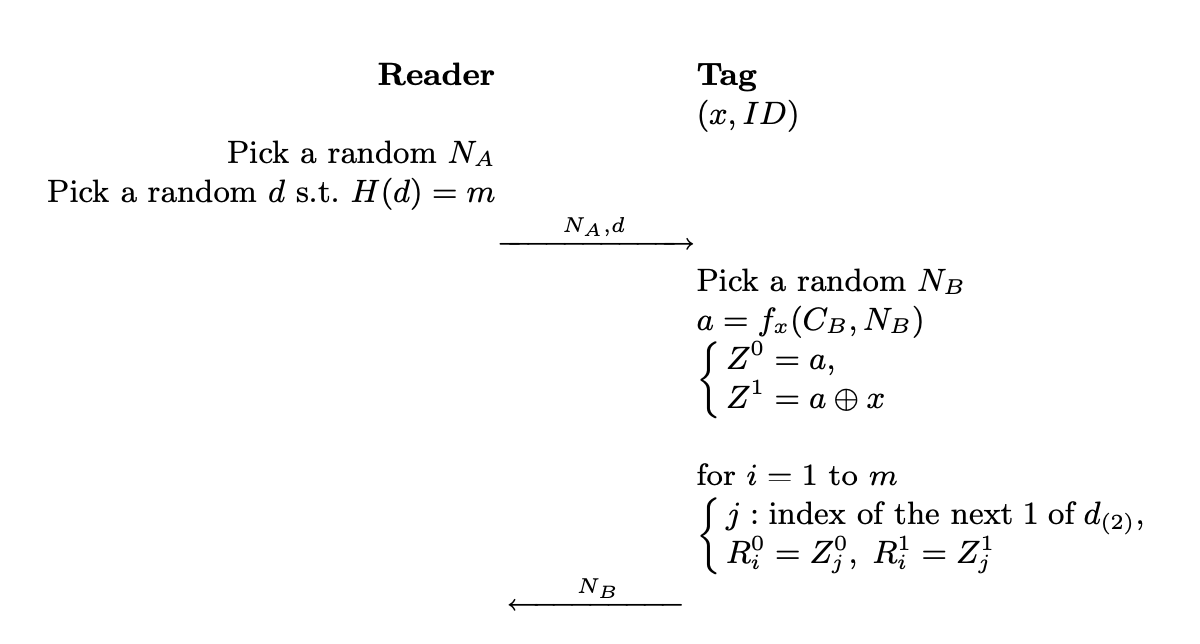
\includegraphics[width=\linewidth]{assets/sk-phase1.png}
    \end{minipage}

    \begin{minipage}[t]{\linewidth}
      \begin{enumerate}
        \item Le lecteur choisit un nonce $N_A$, et $d$ un nombre avec $m$ bits 1.
        \item Le tag choisit un nonce $N_B$, et calcule $a = f_x(C_B, N_B)$ avec sa clé secrète $x$ et $N_B$. ($C_B$ est une constante)
        \item Le tag calcule $Z_0 = a$, $Z_1 = a \oplus x$. Il prépare ensuite les réponses possibles $R_0$ et $R_1$ selon le masque $d$.
        \item Le tag envoie $N_B$ au lecteur.
      \end{enumerate}
    \end{minipage}
  \end{multicols}
\end{frame}

\begin{frame}{Seconde phase : phase rapide}
  \begin{multicols}{2}
    \begin{minipage}[c]{\linewidth}
      \centering
      \bigskip
      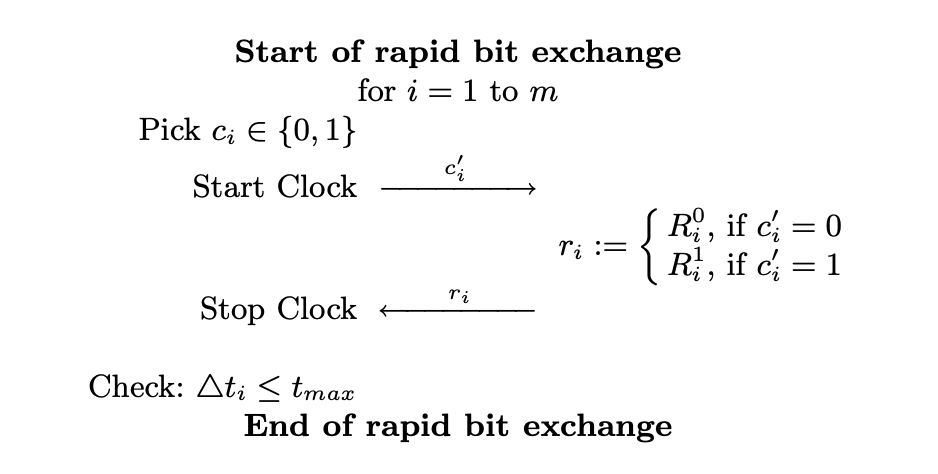
\includegraphics[width=\linewidth]{assets/sk-phase2.png}
    \end{minipage}

    \begin{minipage}[t]{\linewidth}
      \begin{enumerate}
        \item Le lecteur envoie un bit aléatoire $c_i$, et démarre une horloge. Le tag reçoit $c_i'$ (possiblement incorrect).
        \item Le tag répond $r'_i = R_i^{c'_i}$. Le lecteur reçoit $r_i$.
        \item Le lecteur arrête l'horloge, et sauvegarde le délai associé $\Delta t_i$ et la réponse $r_i$ reçue.
      \end{enumerate}
    \end{minipage}
  \end{multicols}
\end{frame}

\begin{frame}{Troisième phase : phase de vérification}
  \begin{multicols}{2}
    \begin{minipage}[c]{\linewidth}
      \centering
      \bigskip
      \bigskip
      \bigskip
      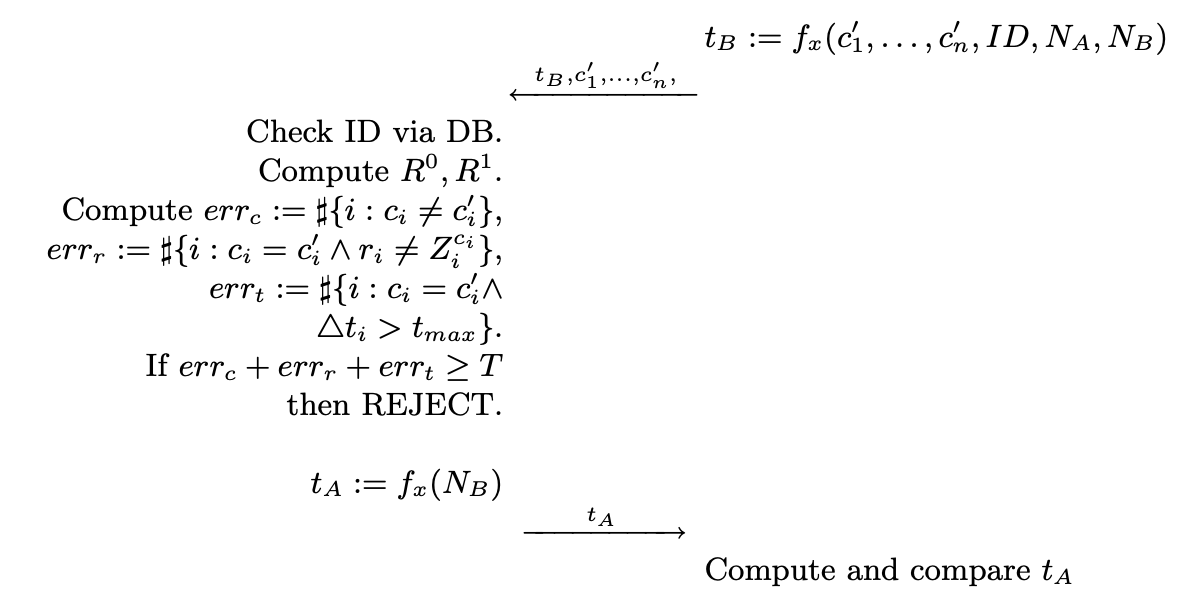
\includegraphics[width=\linewidth]{assets/sk-phase3.png}
    \end{minipage}

    \begin{minipage}[t]{\linewidth}
      \begin{enumerate}
        \item Le lecteur envoie $t_B := f_x(c'_1, \hdots, c'_n, ID, N_A, N_B)$, et les $c'_i$.
        \item Le lecteur cherche dans sa base de tags jusqu'à trouver $(ID, x)$ générant $t_B$.
        \item Le lecteur calcule $R^0$ et $R^1$.
        \item Le lecteur compte les erreurs, si il y en a plus de $T$, échec.
        \item (optionnel) Le lecteur envoie $t_A := f_x(N_B)$ puis le tag le vérifie.
      \end{enumerate}
    \end{minipage}
  \end{multicols}
\end{frame}

\begin{frame}[allowframebreaks]
  \frametitle{Références}
  \printbibliography
\end{frame}

\end{document}
